\subsection{Definition of scenario}
\label{sec:scenario definition}

%Van Notten et al.\ \cite{vannotten2003updated} present an overview of the diversity in the scenarios. Van Notten et al.\ state that ``in view of the observed variety in scenario approaches'', it is assumed ``that there is no `correct' scenario definition or approach. However, the typology uses the following broad working definition: scenarios are descriptions of possible futures that reflect different perspectives on the past, the present and the future.''

% Techniques for scenario development
%Where the contribution of Van Notten et al.\ \cite{vannotten2003updated} relate more to the overall scenario project, Bishop et al.\ \cite{bishop2007scentechniques} focus more on the techniques to produce scenarios, i.e.\ the process of creating scenarios. These scenario development techniques vary from genius forecasting \cite{kahn1962}, event sequences with probability trees \cite{covaliu1995representation} and sensitivity analysis \cite{saltelli2008global}.

% How to apply to real-world traffic scenarios
%If it was not clear yet, the contributions of Van Notten et al.\ \cite{vannotten2003updated} and Bishop et al.\ \cite{bishop2007scentechniques} point out that the notion of scenario is very broad. We are interested in scenarios that can be used in the context of road traffic, which limits the scope of what a scenario is. The description of a scenario by Go and Carroll \cite{go2004blind} is more suited to our needs.
% Definition according to Go and Carroll
Go~and~Carroll~\cite{go2004blind} describe a scenario within the field of system design. They define a scenario as ``a description that contains (1) actors, (2) background information on the actors and assumptions about their environment, (3) actors' goals or objectives, and (4) sequences of actions and events. Some applications may omit one of the elements or they may simply or implicitly express it. Although, in general, the elements of scenarios are the same in any field, the use of scenarios is quite different.'' 

% Definition according to Geyer et al.
Geyer~et~al.~\cite{geyer2014} describe a scenario within the context of automated driving. They use the metaphor of a movie or a storybook for describing a scenario. Geyer~et~al.\ state that ``a scenario includes at least one situation within a scene including the scenery and dynamic elements. However, [a] scenario further includes the ongoing activity of one or both actors.'' For a further explanation of the terms situation, scene and scenery, see \cite{geyer2014}. It is mentioned that the action of the driver and/or automation might be predefined. Here, the meaning of action is not detailed.
%In an example of a so-called crossway scenario, they mention that the course of events might be different. For example, when a car keeps constant speed and then turns right, the scenario consists of one situation. The car might also first decelerate, accelerate and decelerate before turning right. In this case, the scenario consists of four situations.

% Definition according to Ulbrich et al.
Ulbrich~et~al.~\cite{ulbrich2015} also define a scenario in the context of automated driving. They define a scenario as ``the temporal development between several scenes in a sequence of scenes. Every scenario starts with an initial scene. Actions \& events as well as goals \& values may be specified to characterize this temporal development in a scenario. Other than a scene, a scenario spans a certain amount of time.'' They state that actions and events link the different scenes. A further description of actions and events is not given.

% Definition according to Elrofai et al.
Another definition of a scenario in the context of automated driving is given by Elrofai~et~al.~\cite{elrofai2016scenario}. They define scenario as ``the combination of actions and maneuvers of the host vehicle in the passive [i.e., static] environment, and the ongoing activities and maneuvers of the immediate surrounding active [i.e., dynamic] environment for a certain period of time.'' They further mention that the duration of a scenario typically is in the order of seconds.

% "Requirements"
Based on the aforementioned references, the following is concluded about a scenario:

% Order of seconds
\subsubsection{A scenario corresponds to a time interval}
The aforementioned definitions state that a scenario corresponds to a time interval \cite{go2004blind, geyer2014, ulbrich2015, elrofai2016scenario}. Van Notten et al.\ \cite{vannotten2003updated} call such a scenario a chain scenario (``like movies''), as opposed to a snapshot scenario, i.e., a scenario that describes the state at a time instant (``like photos''). The duration of a scenario is in the order of seconds, as explicitly mentioned by Elrofai~et~al.~\cite{elrofai2016scenario}. Though the duration is not mentioned by Ulbrich~et~al.~\cite{ulbrich2015}, the presented example is in the order of seconds. Furthermore, other scenarios regarding (automated) driving are also in the order of seconds, e.g., see \cite{gietelink2006development, zofka2015datadrivetrafficscenarios, roesener2017comprehensive, karaduman2013interactivebehavior, hulshof2013autonomous, englund2016grand}.

% Scenarios consists of one or several events
\subsubsection{A scenario consists of one or several events \cite{vannotten2003updated, go2004blind, geyer2014, ulbrich2015, kahn1962, englund2016grand, schoemaker1993multiple, cuppens2002alert, bach2016modelbased}}
It can be helpful to develop scenarios using events \cite{bishop2007scentechniques}. Thus, a scenario could be defined as a particular sequence of events or, as Kahn \cite{kahn1962} writes, ``a scenario results from an attempt to describe in more or less detail some hypothetical sequence of events''. Furthermore, Geyer~et~al.~\cite{geyer2014} and Ulbrich~et~al.~\cite{ulbrich2015} use the notion of event for describing a scenario, although they do not provide a definition of the term \emph{event}. In Section~\ref{sec:events}, we will elaborate on the notion of \emph{event}.

% Semantically described
\subsubsection{Real-world traffic scenarios are quantitative scenarios}
Regarding the nature of the data, a scenario can be either qualitative or quantitative \cite{vannotten2003updated}. Real-life traffic scenarios are quantitative scenarios, such that they are, e.g., suitable for simulation purposes. A scenario, however, can be described qualitatively, such that it is readable and understandable for human experts. This has become known as a Story-and-Simulation approach \cite{alcamo2001scenarios}. Note that several quantitative scenarios might have the same qualitative description; thus a qualitative description of a scenario does not uniquely define a quantitative scenario. A qualitative description can be regarded as an abstraction of the quantitative scenario.
	
% Some relevance between events
\subsubsection{The time interval of a scenario contains all relevant events}
According to Geyer~et~al.~\cite{geyer2014}, ``the end of a scenario is defined by the first irrelevant situation with respect to the scenario''. In a similar manner, we require that the time interval of a scenario should contain all relevant events. For practical reasons, the term `relevant' must be detailed. First of all, it is important to note that `relevant' is subjective. Therefore, an event is considered to be relevant for the scenario, if it is relevant for the ego vehicle (see Section~\ref{sec:ego vehicle} for a description of the ego vehicle).
% Next to that, an event is regarded as irrelevant, if it is independent of the relevant events.

% Goals (instead of activities)
\subsubsection{A scenario can contain goal(s) of one or multiple actors}
For describing a scenario in real-world data, it is not necessary to describe the goals and as such, Elrofai~et~al.~\cite{elrofai2016scenario} do not mention this. When describing a scenario that an AV has to cope with, however, its goals (i.e., its driving mission \cite{geyer2014}) could be specified rather than its activities \cite{ulbrich2015}. The same holds for other actors within the scenario.
	
% Description of static environment
\subsubsection{A scenario includes the description of the environment}
A scenario should include the description of the static and dynamic environment. It is assumed that the static environment does not change during a scenario. Although this is not a general prerequisite of a scenario, the description of the static environment is often included when speaking about traffic scenarios \cite{geyer2014, ulbrich2015, elrofai2016scenario, ebner2011identifying, schuldt2013effiziente, althoff2017CommonRoad}. Everything that changes during the time interval of a scenario is considered to be part of the dynamic environment. 

% Definition
Hence, we define a scenario as follows.
\begin{definition}[Scenario]\label{def:scenario}
	A scenario is a quantitative description of the ego vehicle, its activities and/or goals, its static environment, and its dynamic environment. From the perspective of the ego vehicle, it contains all relevant events.
\end{definition}

% Describe difference from literature
% - quantitative --> to avoid ambiguous situation and to serve assessment
% - notion of scene not used. Scene follows from description, but is not explicitely used
Definition~\ref{def:scenario} deviates from existing definitions \cite{geyer2014, ulbrich2015, elrofai2016scenario} from the fact that it explicitly mentions that a scenario is quantitative. As a result, a qualitative description of a scenario refers to multiple scenarios. Hence, the qualitative description can be regarded as an abstraction of the quantitative scenarios. A \emph{scenario class} refers to the qualitative description, see Section~\ref{sec:scenario classes}.

Geyer~et~al.~\cite{geyer2014} and Ulbrich~et~al.\cite{ulbrich2015} use the term \emph{scene} to define a scenario, while Definition~\ref{def:scenario} describe the scenes implicitly. Thus the scenes do not have to be described explicitly.

Figure~\ref{fig:scenario} provides a schematic overview of what a scenario contains. As shown in the second row of Figure~\ref{fig:scenario}, a scenario contains a description of the ego vehicle, the dynamic environment and the static environment. As an example, the possible activities of the target vehicle, which is part of the dynamic environment, are detailed by considering the states `heading' and `speed'. The two rows of the activities show more generic descriptions and more detailed descriptions, respectively, of some possible activities.

\begin{figure}
	\centering
	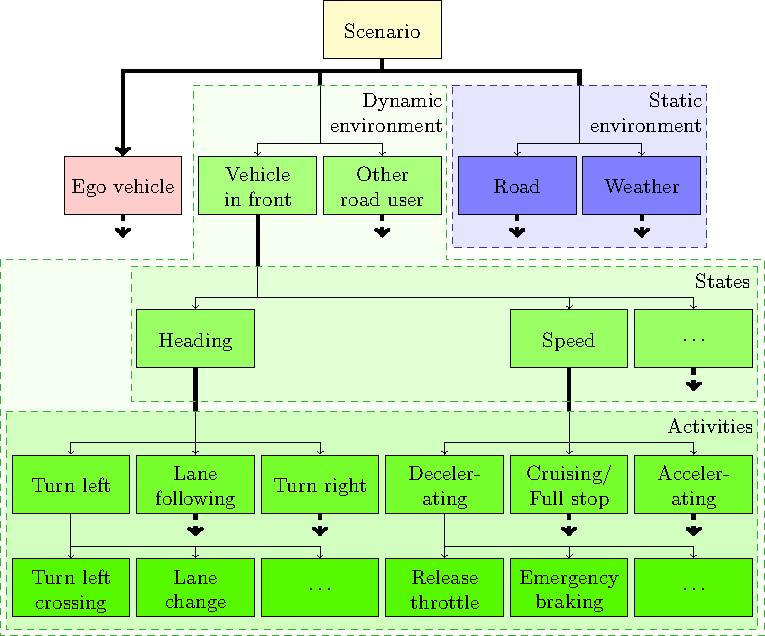
\includegraphics[width=\linewidth]{figures/scenario.pdf}
	\caption{Schematic overview of a scenario.}
	\label{fig:scenario}
	\vspace{\spaceaftercaption}
\end{figure}
